%Presentación examen profesional
%

\documentclass[]{beamer}
\usepackage{babel}
\usepackage{mathtools}
\usepackage{amsthm}
\usepackage{xcolor}
\usepackage[most]{tcolorbox} %para encerrar texto en cajas de colores

%%%% Mis macros %%%%

			%% Secciones:
	
			\newtheorem{teo}{\bf Theorem}
			\newtheorem{lema}{\textbf{Lemma}}
			\newtheorem{prop}{\bf Proposition}
			\newtheorem{obs}{\bf Observation}
			\newtheorem{dem}{\bf Proof}
			\newtheorem{cor}{\bf Corollary}
			\newtheorem{defi}{\bf Definition}
			\newtheorem{ej}{\bf Example}
			\newtheorem{notacion}{\bf Notation}
			\newtheorem{hip}{\bf Hypothesis}

			
			\theoremstyle{definition}
			\newtheorem{nota}{\bf Nota}

			%% Símbolos matemáticos
			\newcommand*{\QEDA}{\null\nobreak\hfill\ensuremath{\blacksquare}}%
			\newcommand*{\QEDB}{\null\nobreak\hfill\ensuremath{\square}}%
			\newcommand{\TODO}[1]{\textcolor{purple}{#1}}
			\newcommand*{\final}{\null\nobreak\hfill\ensuremath{\diamond}}
			\newcommand{\IR}{\mathbb{R}}
			\newcommand{\IC}{\mathbb{C}}
			\newcommand{\IN}{\mathbb{N}}
			\newcommand{\IZ}{\mathbb{Z}}
			\newcommand{\suma}[3]{\sum\limits_{#1}^{#2}#3} %Sumas y series
			\newcommand{\union}[3]{\bigcup\limits_{#1}^{#2}{#3}} %uniones
			\newcommand{\producto}[3]{\prod_{#1}^{#2}{#3}} %productos
			\newcommand{\limite}[2]{\lim\limits_{#1}{#2}} %límites
			\newcommand{\limsu}[2]{\lim\limits_{#1 \rightarrow \infty }#2_{#1}}
			%para límites de sucesiones
			\newcommand{\Om}{\Omega}
			\newcommand{\cali}[1]{\mathcal{#1}} %Letras caligráficas
			\newcommand{\cont}[2]{$\mathcal{C} [#1, #2]$}
			\newcommand{\integ}[3]{\int_{#1}^{#2}{#3}}
			\newcommand{\ldos}{\mathit{l}^{2}}


			\DeclareMathOperator*{\ameboxplus}{{\boxplus}}





\title{La transformada de Haar-Legendre}
\author{Amélie Bernès}

%\usecolortheme{owl}
\usecolortheme[snowy]{owl}
\usetheme{Hannover}
%\useinnertheme{circles}


\title[]{A study and spectral analysis of the discrete Legendre polynomials} 

\author[]{Amélie Bernès \and Moisés Soto Bajo \and Javier Herrera Vega} 

\institute[BUAP]{Benemérita Universidad Autónoma de Puebla \\ \smallskip \textit{ammel.bernes@gmail.com}}

\date[\today]{\today} % Presentation date or conference/meeting name, the optional parameter can contain a shortened version to appear on the bottom of every slide, while the required parameter value is output to the title slide

\begin{document}


% ------------------------------------------------------------ %
% ------------------------------------------------------------ %

\begin{frame}
\titlepage
\end{frame}

% ------------------------------------------------------------ %
% ------------------------------------------------------------ %


% ------------------------------------------------------------ %
% ------------------------------------------------------------ %
\begin{frame}{Outline}
    \tableofcontents
\end{frame}

% ------------------------------------------------------------ %
% ------------------------------------------------------------ %





% ------------------------------------------------------------ %
% ------------------------------------------------------------ %
\section{Motivación}
\begin{frame}
Fijado $n \geq 2$ entero, una \textbf{señal de dimensión $n$} será
representada como un vector $x = (x_{m})_{m=0}^{n-1}$ 
de $\IR^{n}$. La \textbf{gráfica} de $x$
será el conjunto
\[
G_{x} := \{ (m, x_{m}): \hspace{0.2cm} 0 \leq m \leq n-1 \}. 
\]
\pause


\begin{figure}[H]
\centering
	\begin{figure}
		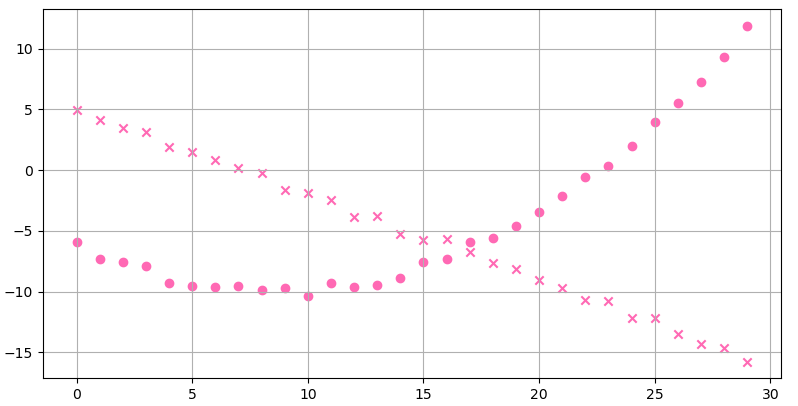
\includegraphics[scale=0.4]{graficasAfinCuadr} 
 	\end{figure}
 \end{figure}

Nos interesa estudiar la forma de la gráfica de una señal, en particular,
saber si parece tener forma de recta o parábola.

\end{frame}

% ------------------------------------------------------------ %
% ------------------------------------------------------------ %






% ------------------------------------------------------------ %
% ------------------------------------------------------------ %
\begin{frame}
Una señal $x \in \IR^{n}$ se dirá \textbf{afín} si su gráfica
$G_{x}$ es la discretización puntual de una recta 
$l : y = mx + b$.
en la malla
\[
\cali{P}_{n} := \{0, 1, \ldots , n-1 \}.
\]

Si la recta es de la forma $l: y = b$, diremos que $x$ es \textbf{constante.}

\begin{figure}[H]
\centering
	\begin{figure}
		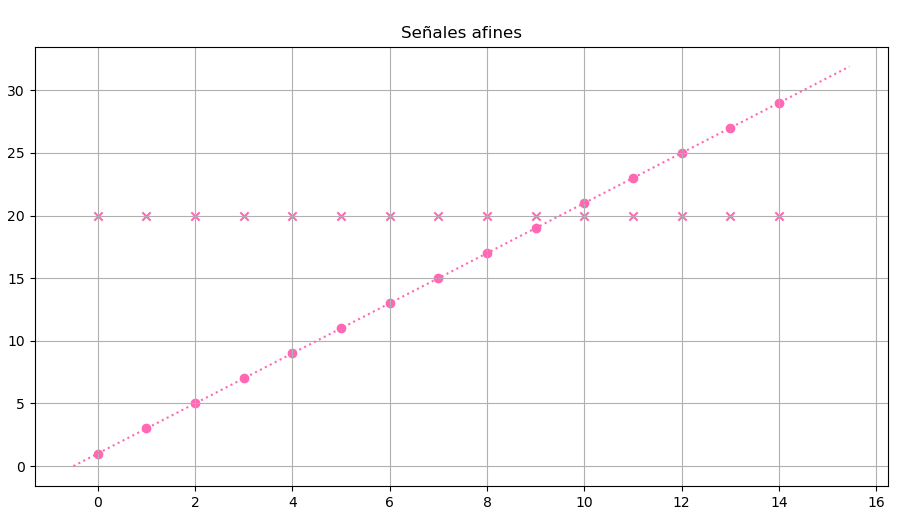
\includegraphics[scale=0.4]{afines}
 	\end{figure}
 \end{figure}


\end{frame}

% ------------------------------------------------------------ %
% ------------------------------------------------------------ %





% ------------------------------------------------------------ %
% ------------------------------------------------------------ %
\begin{frame}
Una señal $x \in \IR^{n}$ se dirá \textbf{cuadrática} si su gráfica
$G_{x}$ es la discretización puntual de una parábola
$l : y = ax^{2} + bx + c$, con $a \neq 0$, en la malla
$\cali{P}_{n}$.

\begin{figure}[H]
\centering
	\begin{figure}
		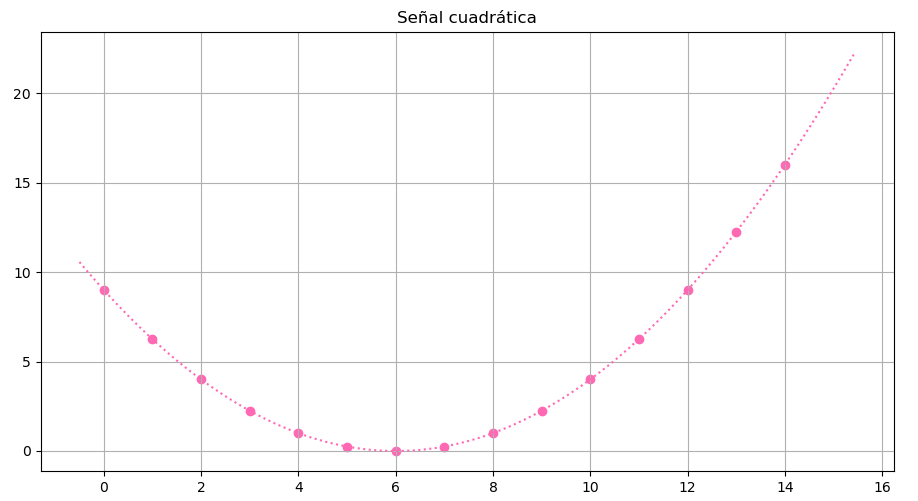
\includegraphics[scale=0.4]{cuadraticas}
 	\end{figure}
 \end{figure}

\end{frame}

% ------------------------------------------------------------ %
% ------------------------------------------------------------ %




% ------------------------------------------------------------ %
% ------------------------------------------------------------ %
\begin{frame}
Fijada una dimensión $n \geq 2$, buscamos una base
$\cali{L}^{n} = \{ \cali{L}^{n,k}: \hspace{0.2cm} 0 \leq k \leq n-1 \}$
de $\IR^{n}$

\begin{itemize}
	\item (\textcolor{red}{Tamaño}) 
	que sea ortonormal, pues así se cumplirá que,
	para toda señal $x \in \IR^{n}$, 
	\[
	x = \suma{k=0}{n-1}{\langle x, \cali{L}^{n,k} \rangle x}
	\hspace{0.2cm} \textit{y} \hspace{0.2cm}
	||x||^{2} = \suma{k=0}{n-1}{\langle x, \cali{L}^{n,k} \rangle^{2}},
	\]
	y
	
	\item (\textcolor{red}{Forma}) para la que sea posible establecer criterios
	sencillos sobre la forma de la gráfica de una señal $x$ en términos
	de la representación de esta respecto a la base $\cali{L}^{n,k}$.
	
\end{itemize}
\end{frame}
% ------------------------------------------------------------ %
% ------------------------------------------------------------ %







% ------------------------------------------------------------ %
% ------------------------------------------------------------ %
\begin{frame}

\begin{figure}[H]
\centering
	\begin{figure}
		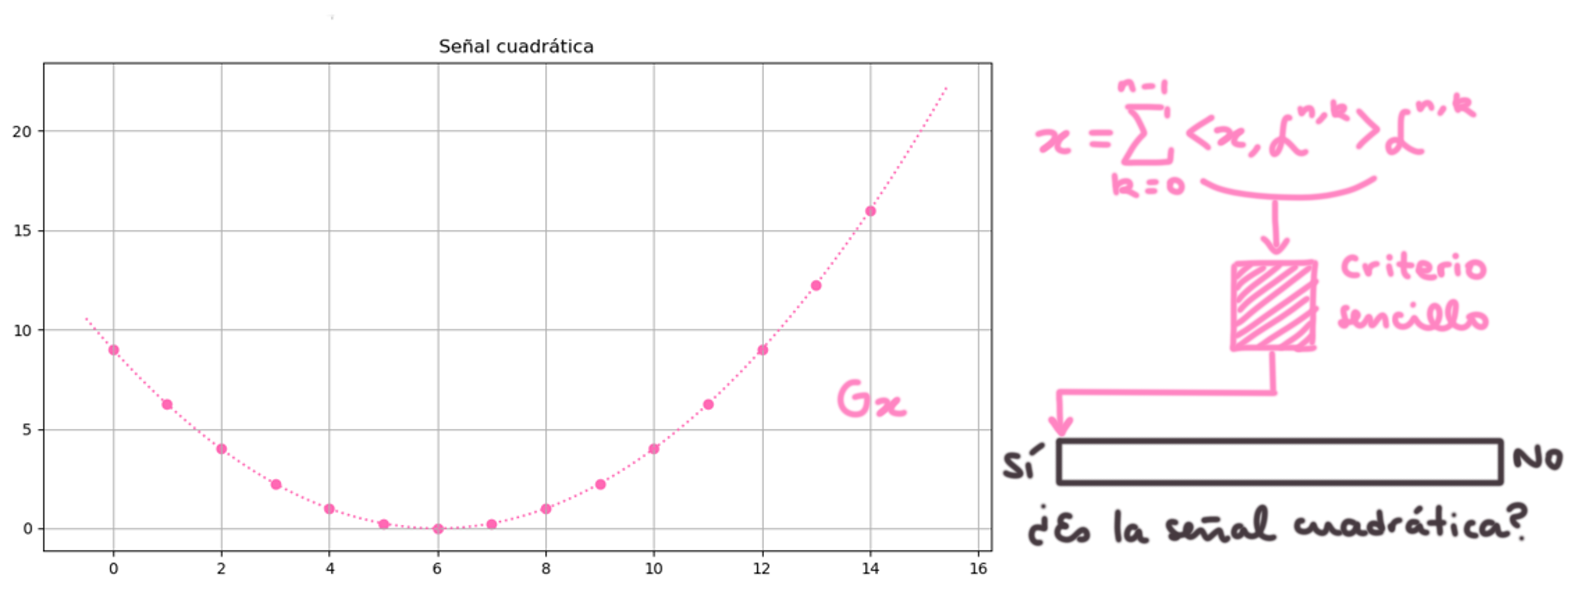
\includegraphics[scale= 0.7 ]{cuadr1}
 	\end{figure}
 \end{figure}

\begin{figure}[H]
\centering
	\begin{figure}
		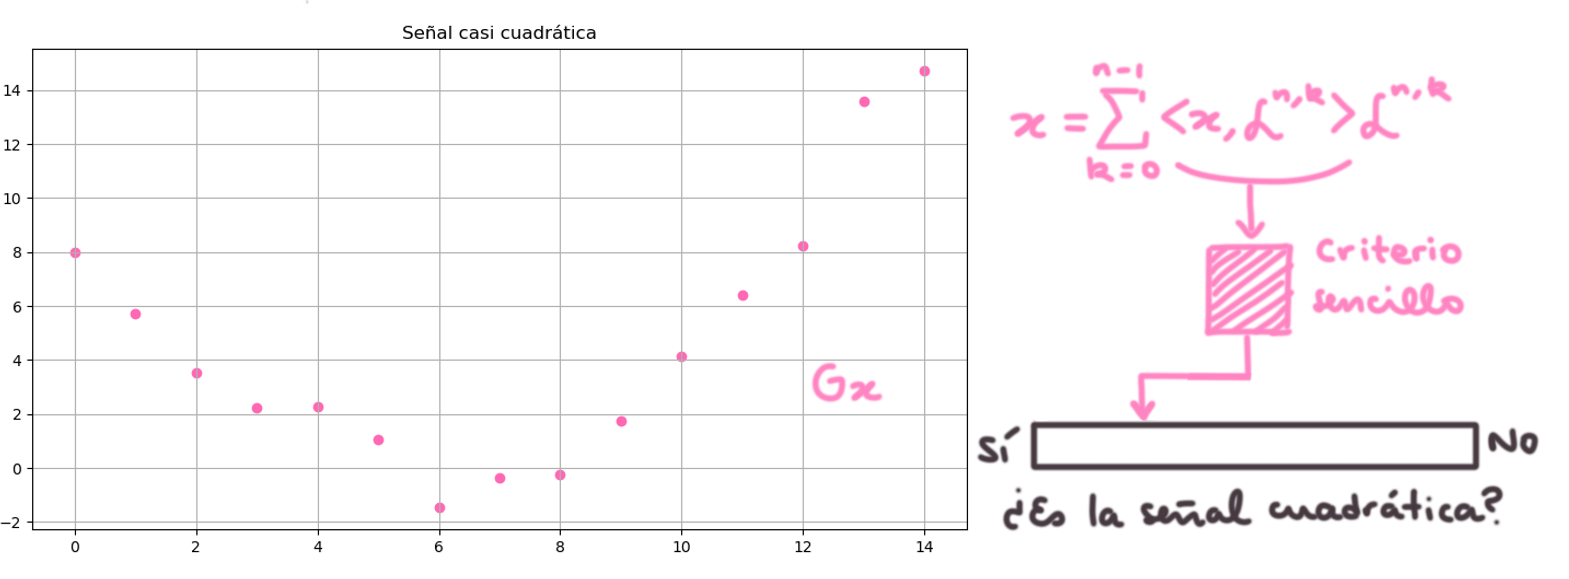
\includegraphics[scale= 0.7]{cuadr2}
 	\end{figure}
 \end{figure}
\end{frame}
% ------------------------------------------------------------ %
% ------------------------------------------------------------ %









\end{document}


%\section{Motivación}
%\section{Espacios de polinomios discretos}
%	\subsection{Espacios $W_{n,k}$}
%	\subsection{Definición del grado de una señal finita}
%\section{Polinomios discretos de Legendre}
%	\subsection{Sobre los PDL en la literatura}
%    \subsection{Construcción}
%    \subsection{Simetrías en las entradas de los PDL}
%   \subsection{Cálculo de los PDL}
%    \subsection{Análisis de señales finitas en base a los PDL}
%\section{Análisis espectral}
%	\subsection{Desarrollo de metodología}
%	\subsection{Resultados del análisis numérico de algunos PDL}
%\section*{Referencias}

